\begin{center}
    \captionof{figure}{Illustration of Within- and Between-Person Effects in Generative Models with $\beta_1 = -0.4$}
    % Top row
    \begin{minipage}[t]{.45\linewidth}
        \centering
        \begin{subfigure}[b]{\linewidth}
            \centering
            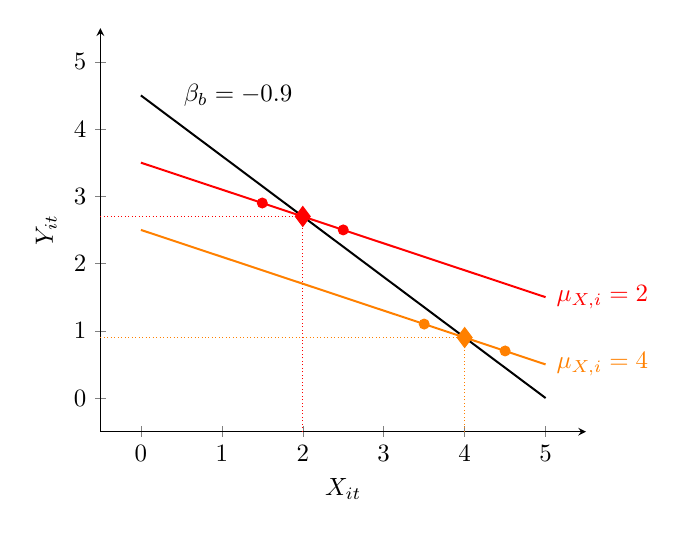
\begin{tikzpicture}[scale=0.9]
                \begin{axis}[
                    axis x line=left, 
                    axis y line=left, 
                    xlabel={$X_{it}$}, ylabel={$Y_{it}$},
                    xmin=0, xmax=5, ymin=0, ymax=5,
                    xtick={0,1,2,3,4,5},
                    ytick={0,1,2,3,4,5},
                    enlargelimits=true,
                    clip=false,
                    xshift=-15mm
                ]
            
                \pgfmathsetmacro{\gammaZero}{4.5}
                \pgfmathsetmacro{\gammaOne}{-0.5}
                \pgfmathsetmacro{\betaOne}{-0.4}
                \pgfmathsetmacro{\betaB}{-0.9}  % gamma01 + beta1
            
                % === Within-person: mu_X = 2 ===
                \addplot[domain=0:5, thick, red] {\gammaZero + \gammaOne*2 + \betaOne*x};
                \addplot[only marks, red] coordinates {
                    (1.5, {4.5 - 0.5*2 - 0.4*1.5})
                    % (2.0, {4.5 - 0.5*2 - 0.4*2.0})
                    (2.5, {4.5 - 0.5*2 - 0.4*2.5})
                };
                \addplot[only marks, mark=diamond*, mark size=4pt, red] coordinates {
                    (2.0, {4.5 - 0.5*2 - 0.4*2.0})
                };
                \addplot[densely dotted, thin, red] coordinates {
                    (2.0, -0.5)
                    (2.0, {4.5 - 0.5*2 - 0.4*2.0})
                };
                \addplot[densely dotted, thin, red] coordinates {
                    (-0.5, {4.5 - 0.5*2 - 0.4*2.0})
                    (2.0, {4.5 - 0.5*2 - 0.4*2.0})
                };
            
                % === Within-person: mu_X = 4 ===
                \addplot[domain=0:5, thick, orange] {\gammaZero + \gammaOne*4 + \betaOne*x};
                \addplot[only marks, orange] coordinates {
                    (3.5, {4.5 - 0.5*4 - 0.4*3.5})
                    % (4.0, {4.5 - 0.5*4 - 0.4*4.0})
                    (4.5, {4.5 - 0.5*4 - 0.4*4.5})
                };
                \addplot[only marks, mark=diamond*, mark size=4pt, orange] coordinates {
                    (4.0, {4.5 - 0.5*4 - 0.4*4.0})
                };
                \addplot[densely dotted, thin, orange] coordinates {
                    (4.0, -0.5)
                    (4.0, {4.5 - 0.5*4 - 0.4*4.0})
                };
                \addplot[densely dotted, thin, orange] coordinates {
                    (-0.5, {4.5 - 0.5*4 - 0.4*4})
                    (4.0, {4.5 - 0.5*4 - 0.4*4.0})
                };
            
                % === Between-person regression line ===
                \addplot[thick, black, domain=0:5] {\gammaZero + \betaB*x};
            
                % === Labels ===
                \node[red] at (axis cs:5.7,1.5) {$\mu_{X,i}=2$};
                \node[orange] at (axis cs:5.7,0.5) {$\mu_{X,i}=4$};
                \node[black] at (axis cs:1.2,4.5) {$\beta_\text{b} = -0.9$};
            
                \end{axis}
            \end{tikzpicture}
            \caption{Continuous X and Y}\label{fig:withinbetween-contxy}
        \end{subfigure}
    \end{minipage}
    \hfill
    \begin{minipage}[t]{.45\linewidth}
        \centering
        \begin{subfigure}[b]{\linewidth}
            \centering

            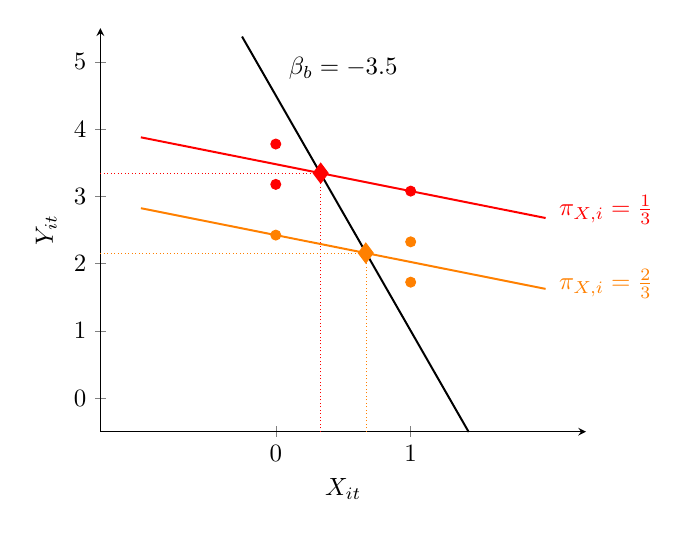
\begin{tikzpicture}[scale=0.9]
                \begin{axis}[
                    axis x line=left, 
                    axis y line=left, 
                    xlabel={$X_{it}$}, ylabel={$Y_{it}$},
                    xmin=-1, xmax=2, ymin=0, ymax=5,
                    xtick={0,1},
                    ytick={0,1,2,3,4,5},
                    enlargelimits=true,
                    clip=false,
                    xshift=-15mm,
                    samples=200,
                    domain=-1:2,
                ]
            
                \pgfmathsetmacro{\gammaZero}{4.5}
                \pgfmathsetmacro{\gammaOne}{-3.1}
                \pgfmathsetmacro{\betaOne}{-0.4}
                \pgfmathsetmacro{\betaB}{-3.5}
            
                % === Person with mu_X = 0.33 ===
                \pgfmathsetmacro{\muXone}{0.33}
                \pgfmathsetmacro{\intOne}{\gammaZero + \gammaOne*\muXone}
                \addplot[thick, red] coordinates {
                    (-1, {\intOne + \betaOne*-1})
                    (2, {\intOne + \betaOne*2})
                };
                \addplot[only marks, mark=diamond*, mark size=4pt, red] coordinates {
                (0.333, {\intOne + \betaOne*0.333})
                };
                \addplot[only marks, red] coordinates {
                    % (0, {\intOne + \betaOne*0})
                    (0, {\intOne + \betaOne*0.75})
                    (0, {\intOne + \betaOne*-0.75})
                    % (1, {\intOne + \betaOne*0.25})
                    (1, {\intOne + \betaOne*1})
                    % (1, {\intOne + \betaOne*1.75})
                };
                \addplot[densely dotted, thin, red] coordinates {
                    (\muXone, -0.5)
                    (\muXone, {\gammaZero + \betaB*\muXone})
                };
                \addplot[densely dotted, thin, red] coordinates {
                    (-1.3, {\gammaZero + \betaB*\muXone})
                    (\muXone, {\gammaZero + \betaB*\muXone})
                };
            
                % === Person with mu_X = 0.67 ===
                \pgfmathsetmacro{\muXtwo}{0.67}
                \pgfmathsetmacro{\intTwo}{\gammaZero + \gammaOne*\muXtwo}
                \addplot[thick, orange] coordinates {
                    (-1, {\intTwo + \betaOne*-1})
                    (2, {\intTwo + \betaOne*2})
                };
                \addplot[only marks, mark=diamond*, mark size=4pt, orange] coordinates {
                (0.667, {\intTwo + \betaOne*0.667})
                };
                \addplot[only marks, orange] coordinates {
                    (0, {\intTwo + \betaOne*0})
                    % (0, {\intTwo + \betaOne*0.75})
                    % (0, {\intTwo + \betaOne*-0.75})
                    (1, {\intTwo + \betaOne*0.25})
                    % (1, {\intTwo + \betaOne*1})
                    (1, {\intTwo + \betaOne*1.75})
                };
                \addplot[densely dotted, thin, orange] coordinates {
                    (\muXtwo, -0.5)
                    (\muXtwo, {\gammaZero + \betaB*\muXtwo})
                };
                \addplot[densely dotted, thin, orange] coordinates {
                    (-1.3, {\gammaZero + \betaB*\muXtwo})
                    (\muXtwo, {\gammaZero + \betaB*\muXtwo})
                };
            
                % === Between-person regression line ===
                \addplot[thick, black, domain=-0.25:1.43] {\gammaZero + \betaB*x};
            
                % === Labels ===
                \node[red] at (axis cs:2.45,2.8) {$\pi_{X,i}=\frac{1}{3}$};
                \node[orange] at (axis cs:2.45,1.7) {$\pi_{X,i}=\frac{2}{3}$};
                \node[black] at (axis cs:0.5,4.9) {$\beta_\text{b} = -3.5$};
            
                \end{axis}
            \end{tikzpicture}
            
            \caption{Binary X and Continuous Y}\label{fig:withinbetween-binxconty}
        \end{subfigure}
    \end{minipage}

    \vskip 1em

    % Bottom row
    \begin{minipage}[t]{.45\linewidth}
        \centering
        \begin{subfigure}[b]{\linewidth}
            \centering

            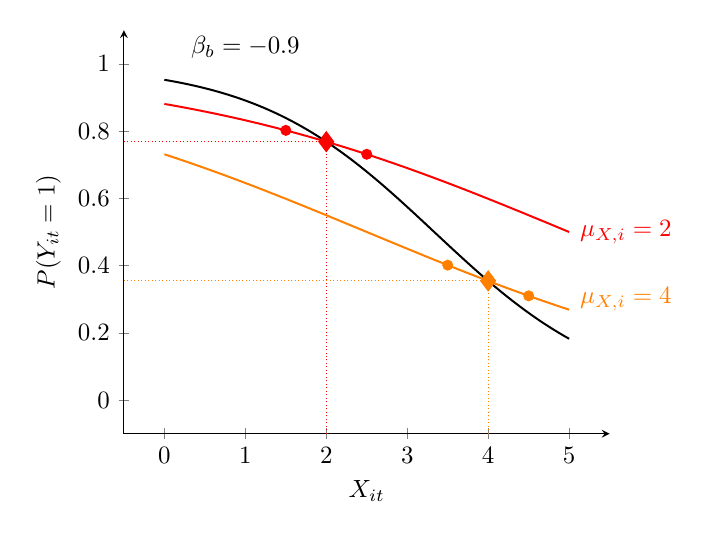
\begin{tikzpicture}[scale=0.9]
            \begin{axis}[
                axis x line=left, axis y line=left,
                xlabel={$X_{it}$}, ylabel={$P(Y_{it} = 1)$},
                xmin=0, xmax=5, ymin=0, ymax=1,
                % legend pos=south west,
                samples=200,
                domain=0:5,
                ytick={0,0.2,0.4,0.6,0.8,1},
                xtick={0,1,2,3,4,5},
                clip=false,
                enlargelimits=true
            ]
            
            % Parameters
            \pgfmathsetmacro{\gammaZero}{3}
            \pgfmathsetmacro{\gammaOne}{-0.5}
            \pgfmathsetmacro{\betaOne}{-0.4}
            \pgfmathsetmacro{\betaB}{-0.9}
            
            % Person 1: mu_X = 2
            \pgfmathsetmacro{\muXone}{2}
            \pgfmathsetmacro{\intOne}{\gammaZero + \gammaOne*\muXone}
            \addplot[red, thick] {1 / (1 + exp(-(\intOne + \betaOne*x)))};
            \addplot[only marks, mark=*, red] coordinates {
                (1.5, {1 / (1 + exp(-(\intOne + \betaOne*1.5)))})
                (2.5, {1 / (1 + exp(-(\intOne + \betaOne*2.5)))})
            };
            \addplot[only marks, mark=diamond*, mark size=4pt, red] coordinates {
                (2, {1 / (1 + exp(-(\intOne + \betaOne*2)))})
            };
            \addplot[densely dotted, thin, red] coordinates {
                (\muXone, -0.1)
                (\muXone, {1 / (1 + exp(-(\intOne + \betaOne*\muXone)))})
            };
            \addplot[densely dotted, thin, red] coordinates {
                (-0.5, {1 / (1 + exp(-(\intOne + \betaOne*\muXone)))})
                (\muXone, {1 / (1 + exp(-(\intOne + \betaOne*\muXone)))})
            };
            
            
            % Person 2: mu_X = 4
            \pgfmathsetmacro{\muXtwo}{4}
            \pgfmathsetmacro{\intTwo}{\gammaZero + \gammaOne*\muXtwo}
            \addplot[orange, thick] {1 / (1 + exp(-(\intTwo + \betaOne*x)))};
            \addplot[only marks, mark=*, orange] coordinates {
                (3.5, {1 / (1 + exp(-(\intTwo + \betaOne*3.5)))})
                (4.5, {1 / (1 + exp(-(\intTwo + \betaOne*4.5)))})
            };
            \addplot[only marks, mark=diamond*, mark size=4pt, orange] coordinates {
                (4, {1 / (1 + exp(-(\intTwo + \betaOne*4)))})
            };
            \addplot[densely dotted, thin, orange] coordinates {
            (\muXtwo, -0.1)
            (\muXtwo, {1 / (1 + exp(-(\intTwo + \betaOne*\muXtwo)))})
            };
            \addplot[densely dotted, thin, orange] coordinates {
            (-0.5, {1 / (1 + exp(-(\intTwo + \betaOne*\muXtwo)))})
            (\muXtwo, {1 / (1 + exp(-(\intTwo + \betaOne*\muXtwo)))})
            };
            
            % Between-person curve
            \addplot[black, thick] {1 / (1 + exp(-(\gammaZero + \betaB*x)))};
        
            % === Labels ===
            \node[red] at (axis cs:5.7,0.5) {$\mu_{X,i}=2$};
            \node[orange] at (axis cs:5.7,0.3) {$\mu_{X,i}=4$};
            \node[black] at (axis cs:1,1.05) {$\beta_\text{b} = -0.9$};
            
            
            \end{axis}
            \end{tikzpicture}
        
            \caption{Continuous X and Binary Y}\label{fig:withinbetween-contxbiny}
        \end{subfigure}
    \end{minipage}
    \hfill
    \begin{minipage}[t]{.45\linewidth}
        \centering
        \begin{subfigure}[b]{\linewidth}
            \centering
            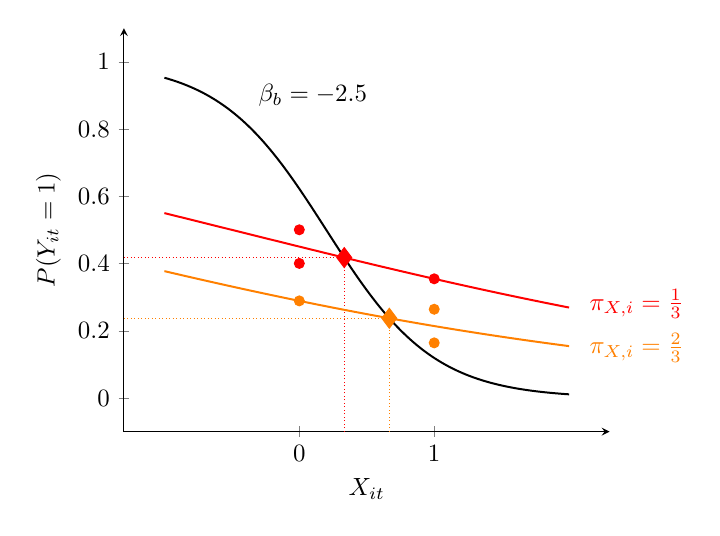
\begin{tikzpicture}[scale=0.9]
            \begin{axis}[
                axis x line=left, axis y line=left,
                xlabel={$X_{it}$}, ylabel={$P(Y_{it} = 1)$},
                xmin=-1, xmax=2, ymin=0, ymax=1,
                % legend pos=south west,
                samples=200,
                domain=-1:2,
                ytick={0,0.2,0.4,0.6,0.8,1},
                xtick={0,1},
                clip=false,
                enlargelimits=true
            ]
            
            % Parameters
            \pgfmathsetmacro{\gammaZero}{0.5}
            \pgfmathsetmacro{\gammaOne}{-2.1}
            \pgfmathsetmacro{\betaOne}{-0.4}
            \pgfmathsetmacro{\betaB}{-2.5}
            
            % Person 1: mu_X = 0.333
            \pgfmathsetmacro{\muXone}{0.333}
            \pgfmathsetmacro{\intOne}{\gammaZero + \gammaOne*\muXone}
            \addplot[red, thick] {1 / (1 + exp(-(\intOne + \betaOne*x)))};
            \addplot[only marks, mark=diamond*, mark size=4pt, red] coordinates {
                (0.333, {1 / (1 + exp(-(\intOne + \betaOne*0.333)))})
            };
            \addplot[only marks, mark=*, red] coordinates {
                % (0, {1 / (1 + exp(-(\intOne + \betaOne*0)))})
                (0, {1 / (1 + exp(-(\intOne + \betaOne*0))) + 0.05})
                (0, {1 / (1 + exp(-(\intOne + \betaOne*0))) - 0.05})
                (1, {1 / (1 + exp(-(\intOne + \betaOne*1)))})
                % (1, {1 / (1 + exp(-(\intOne + \betaOne*1))) + 0.05})
                % (1, {1 / (1 + exp(-(\intOne + \betaOne*1))) - 0.05})
            };
            \addplot[densely dotted, thin, red] coordinates {
                (\muXone, -0.1)
                (\muXone, {1 / (1 + exp(-(\intOne + \betaOne*\muXone)))})
            };
            \addplot[densely dotted, thin, red] coordinates {
                (-1.3, {1 / (1 + exp(-(\intOne + \betaOne*\muXone)))})
                (\muXone, {1 / (1 + exp(-(\intOne + \betaOne*\muXone)))})
            };
            
            % Person 2: mu_X = 0.667
            \pgfmathsetmacro{\muXtwo}{0.667}
            \pgfmathsetmacro{\intTwo}{\gammaZero + \gammaOne*\muXtwo}
            \addplot[orange, thick] {1 / (1 + exp(-(\intTwo + \betaOne*x)))};
            \addplot[only marks, mark=diamond*, mark size=4pt, orange] coordinates {
                (0.667, {1 / (1 + exp(-(\intTwo + \betaOne*0.667)))})
            };
            \addplot[only marks, mark=*, orange] coordinates {
                (0, {1 / (1 + exp(-(\intTwo + \betaOne*0)))})
                % (0, {1 / (1 + exp(-(\intTwo + \betaOne*0))) + 0.05})
                % (0, {1 / (1 + exp(-(\intTwo + \betaOne*0))) - 0.05})
                % (1, {1 / (1 + exp(-(\intTwo + \betaOne*1)))})
                (1, {1 / (1 + exp(-(\intTwo + \betaOne*1))) + 0.05})
                (1, {1 / (1 + exp(-(\intTwo + \betaOne*1))) - 0.05})
            };
            
            \addplot[densely dotted, thin, orange] coordinates {
            (\muXtwo, -0.1)
            (\muXtwo, {1 / (1 + exp(-(\intTwo + \betaOne*\muXtwo)))})
            };
            \addplot[densely dotted, thin, orange] coordinates {
            (-1.3, {1 / (1 + exp(-(\intTwo + \betaOne*\muXtwo)))})
            (\muXtwo, {1 / (1 + exp(-(\intTwo + \betaOne*\muXtwo)))})
            };
            
            % Between-person curve
            \addplot[black, thick] {1 / (1 + exp(-(\gammaZero + \betaB*x)))};
        
            % === Labels ===
            \node[red] at (axis cs:2.5,0.28){$\pi_{X,i}=\frac{1}{3}$};
            \node[orange] at (axis cs:2.5,0.15) {$\pi_{X,i}=\frac{2}{3}$};
            \node[black] at (axis cs:0.1,0.9) {$\beta_\text{b} = -2.5$};
            
            \end{axis}
        \end{tikzpicture}
        \caption{Binary X and Y}\label{fig:withinbetween-binxy}
        \end{subfigure}
    \end{minipage}
    
    \label{fig:path2}

    \vspace{-1cm}
    \begin{flushleft}
    \begin{figurenote}
    Within-person effects ($\beta_1$) and between-person effects ($\beta_b$) are shown for data-generating mechanisms varying by predictor type $X$ (columns) and outcome type $Y$ (rows), each either continuous or binary. For continuous outcomes, relationships are linear; for binary outcomes, the Y-axis reflects the probability of $Y = 1$, and relationships follow a logistic curve. The solid black line denotes the between-person effect; colored lines represent within-person effects for two individuals. Circles are hypothetical observations; diamonds mark where each within-person slope intersects the between-person slope. Thin dotted lines indicate each person's mean on $X$ and $Y$.
    
    % The within-person effects $\beta_1$ and between-person effects $\beta_\text{b}$ illustrated for data-generating mechanisms that vary by predictor type $X$ (columns) and outcome type $Y$ (rows), each either continuous or binary. For continuous outcomes, the relationship between $X$ and $Y$ are linear, whereas for binary outcomes the Y-axis represents a probability of scoring 1, where the effects have a logistic curves.
    % The solid black line represents the \textit{between-person} effect, while the colored solid lines indicate \textit{within-person} effects for two individuals. Circles represent hypothetical observations. Diamonds mark the point where each individual's within-person slope intersects with the between-person slope, and the thin colored dotted lines indicate that individual’s average on on $X$ and on $Y$.
    \end{figurenote}
    \end{flushleft}
\end{center}

% \begin{center}
%     \captionof{figure}{Within- and Between-Person Effects in Data Generating Models with $\beta_\text{w} = -0.4$}
%     % Top row
%     \begin{minipage}[t]{.45\linewidth}
%         \centering
%         \begin{subfigure}[b]{\linewidth}
%             \centering
%             \begin{tikzpicture}
%                 \begin{axis}[
%                     axis x line=left, 
%                     axis y line=left, 
%                     xlabel={$X_{it}$}, ylabel={$Y_{it}$},
%                     xmin=0, xmax=5, ymin=0, ymax=5,
%                     xtick={0,1,2,3,4,5},
%                     ytick={0,1,2,3,4,5},
%                     enlargelimits=true,
%                     clip=false,
%                     xshift=-15mm
%                 ]
            
%                 \pgfmathsetmacro{\gammaZero}{4.5}
%                 \pgfmathsetmacro{\gammaOne}{-0.5}
%                 \pgfmathsetmacro{\betaOne}{-0.4}
%                 \pgfmathsetmacro{\betaB}{-0.9}  % gamma01 + beta1
            
%                 % === Within-person: mu_X = 2 ===
%                 \addplot[domain=0:5, thick, red] {\gammaZero + \gammaOne*2 + \betaOne*x};
%                 \addplot[only marks, red] coordinates {
%                     (1.5, {4.5 - 0.5*2 - 0.4*1.5})
%                     % (2.0, {4.5 - 0.5*2 - 0.4*2.0})
%                     (2.5, {4.5 - 0.5*2 - 0.4*2.5})
%                 };
%                 \addplot[only marks, mark=diamond*, mark size=4pt, red] coordinates {
%                     (2.0, {4.5 - 0.5*2 - 0.4*2.0})
%                 };
%                 \addplot[densely dotted, thin, red] coordinates {
%                     (2.0, -0.5)
%                     (2.0, {4.5 - 0.5*2 - 0.4*2.0})
%                 };
%                 \addplot[densely dotted, thin, red] coordinates {
%                     (-0.5, {4.5 - 0.5*2 - 0.4*2.0})
%                     (2.0, {4.5 - 0.5*2 - 0.4*2.0})
%                 };
            
%                 % === Within-person: mu_X = 4 ===
%                 \addplot[domain=0:5, thick, orange] {\gammaZero + \gammaOne*4 + \betaOne*x};
%                 \addplot[only marks, orange] coordinates {
%                     (3.5, {4.5 - 0.5*4 - 0.4*3.5})
%                     % (4.0, {4.5 - 0.5*4 - 0.4*4.0})
%                     (4.5, {4.5 - 0.5*4 - 0.4*4.5})
%                 };
%                 \addplot[only marks, mark=diamond*, mark size=4pt, orange] coordinates {
%                     (4.0, {4.5 - 0.5*4 - 0.4*4.0})
%                 };
%                 \addplot[densely dotted, thin, orange] coordinates {
%                     (4.0, -0.5)
%                     (4.0, {4.5 - 0.5*4 - 0.4*4.0})
%                 };
%                 \addplot[densely dotted, thin, orange] coordinates {
%                     (-0.5, {4.5 - 0.5*4 - 0.4*4})
%                     (4.0, {4.5 - 0.5*4 - 0.4*4.0})
%                 };
            
%                 % === Between-person regression line ===
%                 \addplot[thick, black, domain=0:5] {\gammaZero + \betaB*x};
            
%                 % === Labels ===
%                 \node[red] at (axis cs:5.7,1.5) {$\mu_{X,i}=2$};
%                 \node[orange] at (axis cs:5.7,0.5) {$\mu_{X,i}=4$};
%                 \node[black] at (axis cs:1.2,4.5) {$\beta_\text{b} = -0.9$};
            
%                 \end{axis}
%             \end{tikzpicture}
%             \caption{Continuous X and Y}\label{fig:withinbetween-contxy}
%         \end{subfigure}
%     \end{minipage}
%     \hfill
%     \begin{minipage}[t]{.45\linewidth}
%         \centering
%         \begin{subfigure}[b]{\linewidth}
%             \centering
%             \begin{tikzpicture}
%             \begin{axis}[
%                 axis x line=left, axis y line=left,
%                 xlabel={$X_{it}$}, ylabel={$P(Y_{it} = 1)$},
%                 xmin=0, xmax=5, ymin=0, ymax=1,
%                 % legend pos=south west,
%                 samples=200,
%                 domain=0:5,
%                 ytick={0,0.2,0.4,0.6,0.8,1},
%                 xtick={0,1,2,3,4,5},
%                 clip=false,
%                 enlargelimits=true
%             ]
            
%             % Parameters
%             \pgfmathsetmacro{\gammaZero}{3}
%             \pgfmathsetmacro{\gammaOne}{-0.5}
%             \pgfmathsetmacro{\betaOne}{-0.4}
%             \pgfmathsetmacro{\betaB}{-0.9}
            
%             % Person 1: mu_X = 2
%             \pgfmathsetmacro{\muXone}{2}
%             \pgfmathsetmacro{\intOne}{\gammaZero + \gammaOne*\muXone}
%             \addplot[red, thick] {1 / (1 + exp(-(\intOne + \betaOne*x)))};
%             \addplot[only marks, mark=*, red] coordinates {
%                 (1.5, {1 / (1 + exp(-(\intOne + \betaOne*1.5)))})
%                 (2.5, {1 / (1 + exp(-(\intOne + \betaOne*2.5)))})
%             };
%             \addplot[only marks, mark=diamond*, mark size=4pt, red] coordinates {
%                 (2, {1 / (1 + exp(-(\intOne + \betaOne*2)))})
%             };
%             \addplot[densely dotted, thin, red] coordinates {
%                 (\muXone, -0.1)
%                 (\muXone, {1 / (1 + exp(-(\intOne + \betaOne*\muXone)))})
%             };
%             \addplot[densely dotted, thin, red] coordinates {
%                 (-0.5, {1 / (1 + exp(-(\intOne + \betaOne*\muXone)))})
%                 (\muXone, {1 / (1 + exp(-(\intOne + \betaOne*\muXone)))})
%             };
            
            
%             % Person 2: mu_X = 4
%             \pgfmathsetmacro{\muXtwo}{4}
%             \pgfmathsetmacro{\intTwo}{\gammaZero + \gammaOne*\muXtwo}
%             \addplot[orange, thick] {1 / (1 + exp(-(\intTwo + \betaOne*x)))};
%             \addplot[only marks, mark=*, orange] coordinates {
%                 (3.5, {1 / (1 + exp(-(\intTwo + \betaOne*3.5)))})
%                 (4.5, {1 / (1 + exp(-(\intTwo + \betaOne*4.5)))})
%             };
%             \addplot[only marks, mark=diamond*, mark size=4pt, orange] coordinates {
%                 (4, {1 / (1 + exp(-(\intTwo + \betaOne*4)))})
%             };
%             \addplot[densely dotted, thin, orange] coordinates {
%             (\muXtwo, -0.1)
%             (\muXtwo, {1 / (1 + exp(-(\intTwo + \betaOne*\muXtwo)))})
%             };
%             \addplot[densely dotted, thin, orange] coordinates {
%             (-0.5, {1 / (1 + exp(-(\intTwo + \betaOne*\muXtwo)))})
%             (\muXtwo, {1 / (1 + exp(-(\intTwo + \betaOne*\muXtwo)))})
%             };
            
%             % Between-person curve
%             \addplot[black, thick] {1 / (1 + exp(-(\gammaZero + \betaB*x)))};
        
%             % === Labels ===
%             \node[red] at (axis cs:5.7,0.5) {$\mu_{X,i}=2$};
%             \node[orange] at (axis cs:5.7,0.3) {$\mu_{X,i}=4$};
%             \node[black] at (axis cs:1,1.05) {$\beta_\text{b} = -0.9$};
            
            
%             \end{axis}
%         \end{tikzpicture}
%             \caption{Continuous X and Binary Y}\label{fig:withinbetween-contxbiny}
%         \end{subfigure}
%     \end{minipage}

%     \vskip 1em

%     % Bottom row
%     \begin{minipage}[t]{.45\linewidth}
%         \centering
%         \begin{subfigure}[b]{\linewidth}
%             \centering
%             \begin{tikzpicture}
%                 \begin{axis}[
%                     axis x line=left, 
%                     axis y line=left, 
%                     xlabel={$X_{it}$}, ylabel={$Y_{it}$},
%                     xmin=-1, xmax=2, ymin=0, ymax=5,
%                     xtick={0,1},
%                     ytick={0,1,2,3,4,5},
%                     enlargelimits=true,
%                     clip=false,
%                     xshift=-15mm,
%                     samples=200,
%                     domain=-1:2,
%                 ]
            
%                 \pgfmathsetmacro{\gammaZero}{4.5}
%                 \pgfmathsetmacro{\gammaOne}{-3.1}
%                 \pgfmathsetmacro{\betaOne}{-0.4}
%                 \pgfmathsetmacro{\betaB}{-3.5}
            
%                 % === Person with mu_X = 0.33 ===
%                 \pgfmathsetmacro{\muXone}{0.33}
%                 \pgfmathsetmacro{\intOne}{\gammaZero + \gammaOne*\muXone}
%                 \addplot[thick, red] coordinates {
%                     (-1, {\intOne + \betaOne*-1})
%                     (2, {\intOne + \betaOne*2})
%                 };
%                 \addplot[only marks, mark=diamond*, mark size=4pt, red] coordinates {
%                 (0.333, {\intOne + \betaOne*0.333})
%                 };
%                 \addplot[only marks, red] coordinates {
%                     % (0, {\intOne + \betaOne*0})
%                     (0, {\intOne + \betaOne*0.75})
%                     (0, {\intOne + \betaOne*-0.75})
%                     % (1, {\intOne + \betaOne*0.25})
%                     (1, {\intOne + \betaOne*1})
%                     % (1, {\intOne + \betaOne*1.75})
%                 };
%                 \addplot[densely dotted, thin, red] coordinates {
%                     (\muXone, -0.5)
%                     (\muXone, {\gammaZero + \betaB*\muXone})
%                 };
%                 \addplot[densely dotted, thin, red] coordinates {
%                     (-1.3, {\gammaZero + \betaB*\muXone})
%                     (\muXone, {\gammaZero + \betaB*\muXone})
%                 };
            
%                 % === Person with mu_X = 0.67 ===
%                 \pgfmathsetmacro{\muXtwo}{0.67}
%                 \pgfmathsetmacro{\intTwo}{\gammaZero + \gammaOne*\muXtwo}
%                 \addplot[thick, orange] coordinates {
%                     (-1, {\intTwo + \betaOne*-1})
%                     (2, {\intTwo + \betaOne*2})
%                 };
%                 \addplot[only marks, mark=diamond*, mark size=4pt, orange] coordinates {
%                 (0.667, {\intTwo + \betaOne*0.667})
%                 };
%                 \addplot[only marks, orange] coordinates {
%                     (0, {\intTwo + \betaOne*0})
%                     % (0, {\intTwo + \betaOne*0.75})
%                     % (0, {\intTwo + \betaOne*-0.75})
%                     (1, {\intTwo + \betaOne*0.25})
%                     % (1, {\intTwo + \betaOne*1})
%                     (1, {\intTwo + \betaOne*1.75})
%                 };
%                 \addplot[densely dotted, thin, orange] coordinates {
%                     (\muXtwo, -0.5)
%                     (\muXtwo, {\gammaZero + \betaB*\muXtwo})
%                 };
%                 \addplot[densely dotted, thin, orange] coordinates {
%                     (-1.3, {\gammaZero + \betaB*\muXtwo})
%                     (\muXtwo, {\gammaZero + \betaB*\muXtwo})
%                 };
            
%                 % === Between-person regression line ===
%                 \addplot[thick, black, domain=-0.25:1.43] {\gammaZero + \betaB*x};
            
%                 % === Labels ===
%                 \node[red] at (axis cs:2.45,2.8) {$\pi_{X,i}=\frac{1}{3}$};
%                 \node[orange] at (axis cs:2.45,1.7) {$\pi_{X,i}=\frac{2}{3}$};
%                 \node[black] at (axis cs:0.5,4.9) {$\beta_\text{b} = -3.5$};
            
%                 \end{axis}
%             \end{tikzpicture}
%             \caption{Binary X and Continuous Y}\label{fig:withinbetween-binxconty}
%         \end{subfigure}
%     \end{minipage}
%     \hfill
%     \begin{minipage}[t]{.45\linewidth}
%         \centering
%         \begin{subfigure}[b]{\linewidth}
%             \centering
%             \begin{tikzpicture}
%             \begin{axis}[
%                 axis x line=left, axis y line=left,
%                 xlabel={$X_{it}$}, ylabel={$P(Y_{it} = 1)$},
%                 xmin=-1, xmax=2, ymin=0, ymax=1,
%                 % legend pos=south west,
%                 samples=200,
%                 domain=-1:2,
%                 ytick={0,0.2,0.4,0.6,0.8,1},
%                 xtick={0,1},
%                 clip=false,
%                 enlargelimits=true
%             ]
            
%             % Parameters
%             \pgfmathsetmacro{\gammaZero}{0.5}
%             \pgfmathsetmacro{\gammaOne}{-2.1}
%             \pgfmathsetmacro{\betaOne}{-0.4}
%             \pgfmathsetmacro{\betaB}{-2.5}
            
%             % Person 1: mu_X = 0.333
%             \pgfmathsetmacro{\muXone}{0.333}
%             \pgfmathsetmacro{\intOne}{\gammaZero + \gammaOne*\muXone}
%             \addplot[red, thick] {1 / (1 + exp(-(\intOne + \betaOne*x)))};
%             \addplot[only marks, mark=diamond*, mark size=4pt, red] coordinates {
%                 (0.333, {1 / (1 + exp(-(\intOne + \betaOne*0.333)))})
%             };
%             \addplot[only marks, mark=*, red] coordinates {
%                 % (0, {1 / (1 + exp(-(\intOne + \betaOne*0)))})
%                 (0, {1 / (1 + exp(-(\intOne + \betaOne*0))) + 0.05})
%                 (0, {1 / (1 + exp(-(\intOne + \betaOne*0))) - 0.05})
%                 (1, {1 / (1 + exp(-(\intOne + \betaOne*1)))})
%                 % (1, {1 / (1 + exp(-(\intOne + \betaOne*1))) + 0.05})
%                 % (1, {1 / (1 + exp(-(\intOne + \betaOne*1))) - 0.05})
%             };
%             \addplot[densely dotted, thin, red] coordinates {
%                 (\muXone, -0.1)
%                 (\muXone, {1 / (1 + exp(-(\intOne + \betaOne*\muXone)))})
%             };
%             \addplot[densely dotted, thin, red] coordinates {
%                 (-1.3, {1 / (1 + exp(-(\intOne + \betaOne*\muXone)))})
%                 (\muXone, {1 / (1 + exp(-(\intOne + \betaOne*\muXone)))})
%             };
            
%             % Person 2: mu_X = 0.667
%             \pgfmathsetmacro{\muXtwo}{0.667}
%             \pgfmathsetmacro{\intTwo}{\gammaZero + \gammaOne*\muXtwo}
%             \addplot[orange, thick] {1 / (1 + exp(-(\intTwo + \betaOne*x)))};
%             \addplot[only marks, mark=diamond*, mark size=4pt, orange] coordinates {
%                 (0.667, {1 / (1 + exp(-(\intTwo + \betaOne*0.667)))})
%             };
%             \addplot[only marks, mark=*, orange] coordinates {
%                 (0, {1 / (1 + exp(-(\intTwo + \betaOne*0)))})
%                 % (0, {1 / (1 + exp(-(\intTwo + \betaOne*0))) + 0.05})
%                 % (0, {1 / (1 + exp(-(\intTwo + \betaOne*0))) - 0.05})
%                 % (1, {1 / (1 + exp(-(\intTwo + \betaOne*1)))})
%                 (1, {1 / (1 + exp(-(\intTwo + \betaOne*1))) + 0.05})
%                 (1, {1 / (1 + exp(-(\intTwo + \betaOne*1))) - 0.05})
%             };
            
%             \addplot[densely dotted, thin, orange] coordinates {
%             (\muXtwo, -0.1)
%             (\muXtwo, {1 / (1 + exp(-(\intTwo + \betaOne*\muXtwo)))})
%             };
%             \addplot[densely dotted, thin, orange] coordinates {
%             (-1.3, {1 / (1 + exp(-(\intTwo + \betaOne*\muXtwo)))})
%             (\muXtwo, {1 / (1 + exp(-(\intTwo + \betaOne*\muXtwo)))})
%             };
            
%             % Between-person curve
%             \addplot[black, thick] {1 / (1 + exp(-(\gammaZero + \betaB*x)))};
        
%             % === Labels ===
%             \node[red] at (axis cs:2.5,0.28){$\pi_{X,i}=\frac{1}{3}$};
%             \node[orange] at (axis cs:2.5,0.15) {$\pi_{X,i}=\frac{2}{3}$};
%             \node[black] at (axis cs:0.1,0.9) {$\beta_\text{b} = -2.5$};
            
%             \end{axis}
%         \end{tikzpicture}
%         \caption{Binary X and Y}\label{fig:withinbetween-binxy}
%         \end{subfigure}
%     \end{minipage}
    
%     \label{fig:path2}

%     % \vspace{-2cm}
%     \begin{flushleft}
%     \begin{figurenote}
%     The solid black line represents the \textit{between-person} effect, while the colored solid lines indicate \textit{within-person} effects for each individual. Circles represent hypothetical observations. Diamonds mark the point where each individual's within-person slope intersects with the between-person slope, and the thin colored dotted lines indicate that individual’s average on on $X$ and on $Y$.
%     \end{figurenote}
%     \end{flushleft}
% \end{center}
